\section{Методы обеспечения качества программного обеспечения}

Существует две основных группы подходов к разработке качественного программного
обеспечения.

\subsection{Подходы, основанные на синтезе ПО} % (fold)

Данная группа основывается на использовании различных формализаций и модельных
представлений во время проектирования архитектуры программной системы. Таким
образом, путем дополнительных усилий на начальном этапе разработки продукта,
можно минимизировать возможность появления ошибок в дальнейших этапах жизненного
цикла.

В данном подходе применяются:

\begin{itemize}
    \item формальные спецификации.
    \item формальные и неформальные описания различных аспектов программной
    системы.
    \item архитектурные шаблоны и стили.
    \item паттерны проектирования.
    \item генераторы шаблонов программ.
    \item генераторы программ.
    \item контрактное программирование.
    \item аннотирование программ.
    \item верификация моделей программ с использованием частичных спецификаций.
    \item использование моделей предметной области для автоматизации
    тестирования программ.
\end{itemize}

\subsection{Подходы, основанные на анализе уже созданного ПО} % (fold)

Данная группа подходов предназначена для повышения качества уже созданного ПО.
Актуальность этой задачи чрезвычайно высока, так как к данному моменту уже
создано огромное количество программных систем, многие из которых имеют проблемы
с уровнем качества, которые проявляются в виде различных ошибок и сбоев.

Предполагается, что уже имеется разработанное программное обеспечение, и
необходимо оценить и повысить его качество. Проверка может заключаться либо в
доказательстве того, что программа соответствует предъявленным функциональным и
нефункциональным требованиям, либо в приведении контрпримеров, показывающих
несоответствие программы этим требованиям.

\newpage
\subsection{Классификация методов обеспечения качества} % (fold)

Обычно выделяют следующие базовые классификации методов обеспечения качества:

\begin{figure}[h!]
    \begin{center}
        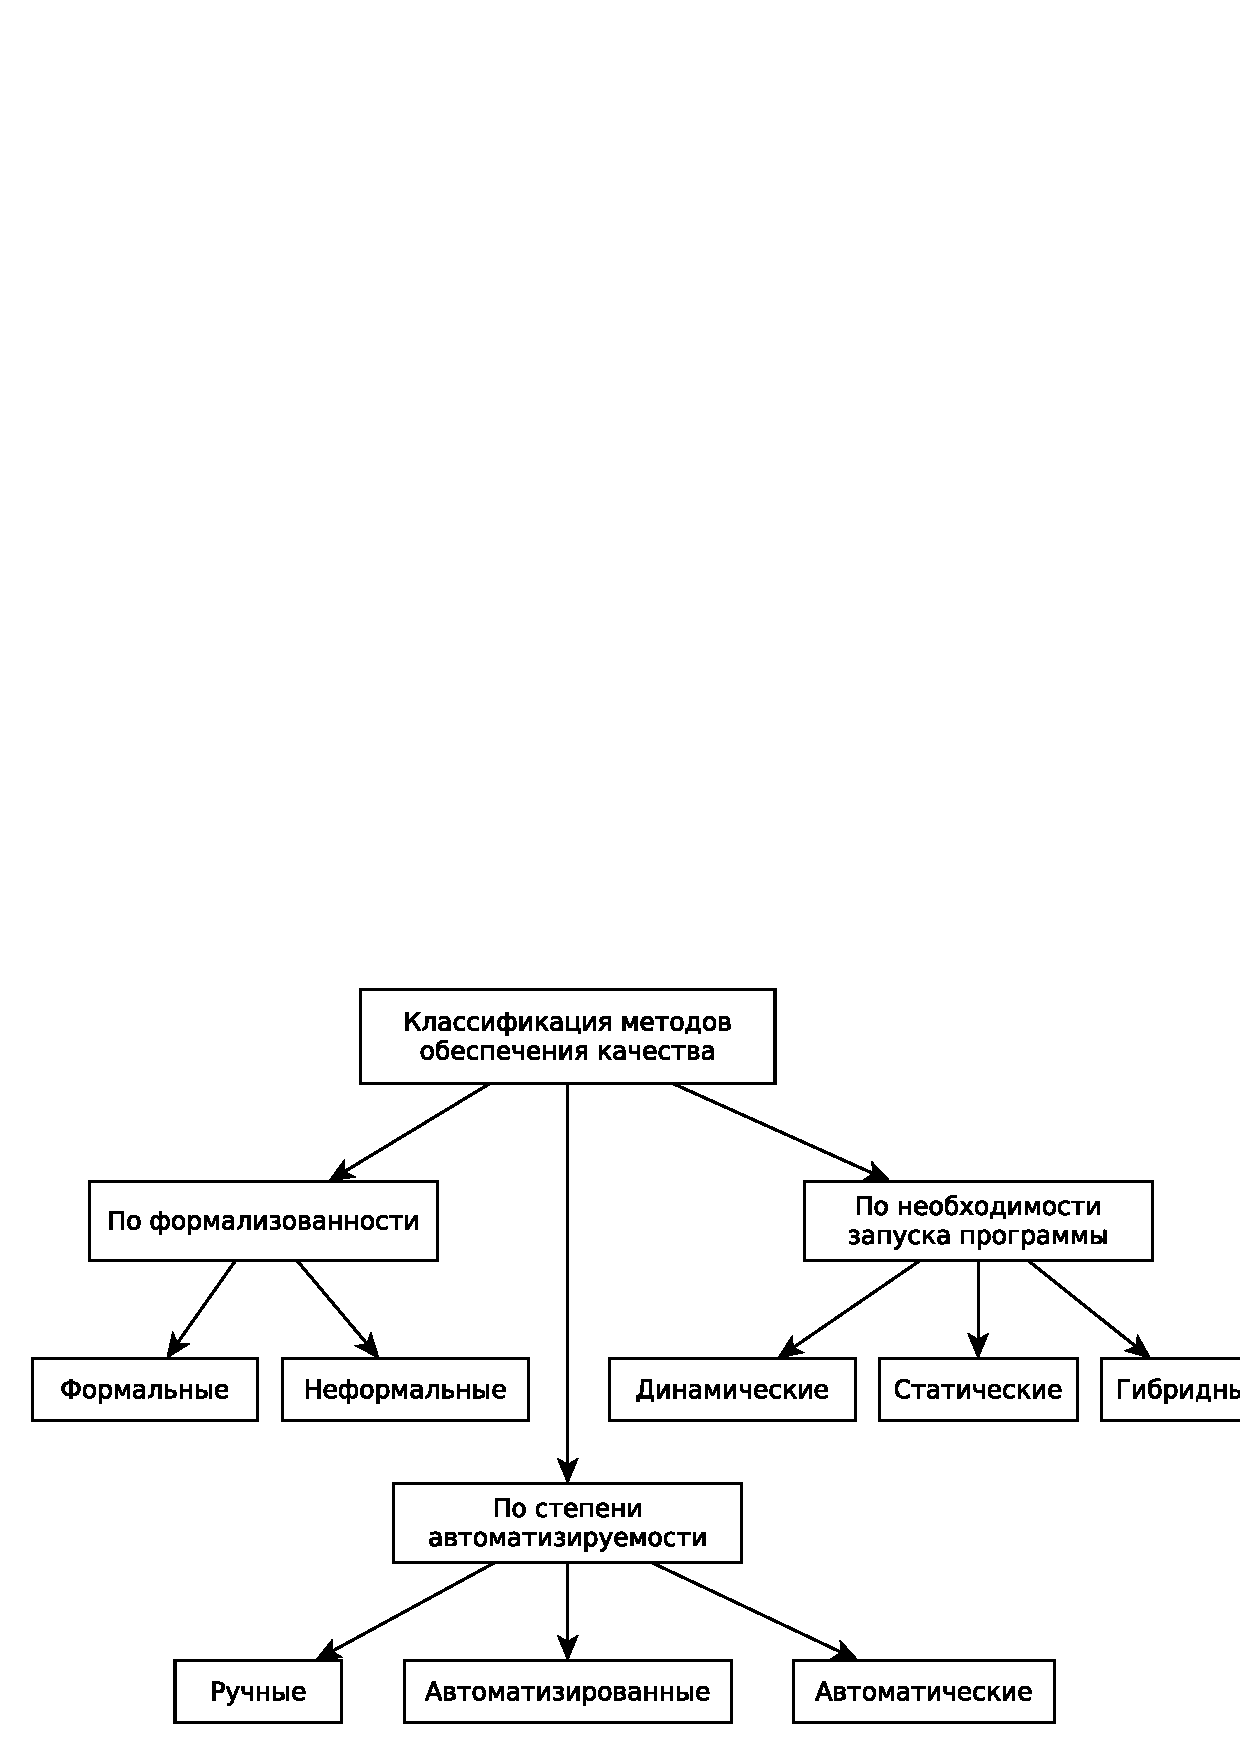
\includegraphics[width=\textwidth]{img/verification_classification.png}
    \end{center}
    \caption{Схема используемой классификации методов верификации}
    \label{fig:figure3}
\end{figure}

\subsubsection{Экспертиза} % (fold)

От других методов верификации экспертизу отличает возможность выполнять ее,
используя только сами артефакты жизненного цикла, а не их модели или результаты
работы, как в формальных и динамических методах. Она позволяет выявлять
практически любые виды ошибок, причем делать это на этапе подготовки
соответствующего артефакта. В то же время она не может быть автоматизирована и
требует активного участия людей.

\subsubsection{Статический анализ} % (fold)

Статический анализ - набор методов, направленный на статический поиск ошибок в
исследуемой программе.

От остальных методов верификации его отделяет то, что статический анализ
позволяет обнаруживать ошибки, вносимые на стадии кодирования. Это связано с
тем, что среди анализируемых артефактов отсутствует спецификация программы, а
это значит, что  анализатор ничего не может знать о том, что делает программа.
Однако, благодаря этому, статический анализ можно полностью автоматизировать.

\subsubsection{Формальные методы} % (fold)

Данные методы использует формальные модели требований, поведения ПО и его
окружения для анализа свойств ПО. К таким методам относятся, например,
дедуктивная верификация, проверка моделей и абстрактная интерпретация.

Эти методы можно применить только к тем свойствам, которые можно выразить в
рамках некоторой математической модели. Построение этой модели не
автоматизируется, а провести анализ таких моделей может лишь специалист. Однако
сама проверка свойств может быть автоматизирована и позволяет находить даже
самые сложные ошибки.

\subsubsection{Динамические методы} % (fold)

Динамические методы используются для анализа и оценки свойств программной
системы по результатам ее реальной работы. Одними из таких методов
являются тестирование и анализ трасс исполнения.

Для применения данных методов необходимо иметь работающую систему (или ее
прототип),  поэтому их нельзя использовать на ранних стадиях разработки. Также
данные методы позволяют найти только те ошибки в ПО, которые проявляются в его
работе.

\subsubsection{Синтетические методы} % (fold)

Данные методы объединяют в себе элементы некоторых способов повышения качества,
описанных выше. Например, существуют динамические методы, использующие элементы
формальных - тестирование на основе моделей (model driven testing) и мониторинг
формальных свойств (runtime verification). Цель таких методов - объединить
преимущества уже используемых подходов.
